%!TEX root = ../../Master.tex
\subsubsection{CrustCrawler}
\label{subsub: CrustCrawler}

Klassen CrustCrawler er en klasse til håndtering af armens positionering. Den har til formål at fortolke det koordinat som fås fra \textbf{block} klassen, og udregne vinkelpositionerne for robotarmens led, således at det er muligt for armen at gribe klodsen.\\

\textbf{inverse\_kinematics\_point}\\
Funktionen har til formål at udregne og bestemme robotarmens ledvinkler på baggrund af det bestemte midtpunkt for klodserne. Den tager et input (self, x, y, z) som beskriver et punkt for klodserne i rummet, P(x, y, z). Ud fra det bestemte punkt er det muligt at finde positionen til end-effektoren. x, y, z bruges til at beregne $q_1$, $q_2$, $q_3$. Hver q-parameter beskriver en ledvinkel for det tilsvarende led. Udregningen af parametrene kan ses i \autoref{inverse kinematics funktion}\\

Parametrene $r^2, s, D$ er geometriske parametre som anvendes til at bestemme $q_2$ og $q_3$. Nedenfor er det illustreret i \autoref{fig:geometric_approach}, hvordan parametrene tolkes.\\

\begin{figure}[h]
\centering
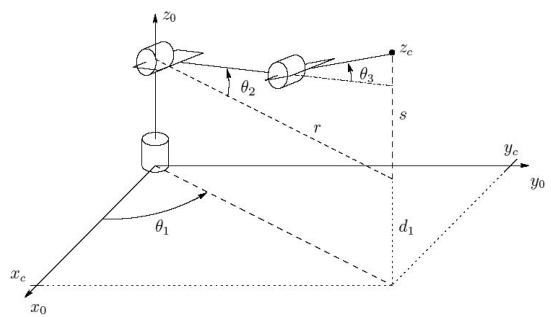
\includegraphics[scale=0.4]{images/geometric_approach}
\caption{Geometrisk bestemmelse af position.}
\label{fig:geometric_approach}
\end{figure}

\newpage
\textbf{inverse\_kinematics\_block}\\
Funktionen har til opgave at bestemme orienteringen af gripperen så den kan gribe klodsen. Dette sker efter at centrum er fundet. Den kalder funktionen \textbf{find\_orientation} som har fundet den mindste $q_4$-værdi som gør at gripperen skal roteres mindst muligt.

\begin{lstlisting}[caption=inverse\_kinematics funktion, label=inverse kinematics funktion, language=Python]
    def inverse_kinematics_block(self, x, y, z, block):
        d1 = 10.0  # cm (height of 2nd joint)
        a1 = 0.0   # (distance along "y-axis" to 2nd joint)
        a2 = 20.0  # (distance between 2nd and 3rd joints)
        d4 = 20.0  # (distance from 3rd joint to gripper center - all inclusive, ie. also 4th joint)

        q1 = atan2(y, x)

        # calculation of q2 and q3
        r2 = (x - a1 * cos(q1)) ** 2 + (y - a1 * sin(q1)) ** 2
        s = z - d1
        D = (r2 + s ** 2 - a2 ** 2 - d4 ** 2) / (2 * a2 * d4)

        q3 = atan2(-sqrt(1 - D ** 2), D)

        q2 = atan2(s, sqrt(r2)) - atan2(d4 * sin(q3), a2 + d4 * cos(q3)) - pi / 2

        q4 = - block.find_orientation(q1)

        return q1, q2, q3, q4
\end{lstlisting}

\textbf{move\_to\_point}\\
Funktionen \textbf{move\_to\_point} har til formål generere den sti af punkter som robotarmen skal følge på baggrund af de bestemte positionsværdier i \textbf{inverse\_kinematics\_point}. Den anvender ROS specifikke kommandoer til at bestemme motorerenes position, hastighed og udførselstid. på \autoref{move to point funktion}\\

Dette foregår altsammen igennem \textbf{JointTrajectoryPoint}, som sætter positionerne til de bestemte værdier i \textbf{inverse\_kinematics\_point} samt begrænsningerne for hvert motorleds acceleration og hastighed. \textbf{JointTrajectory} er ansvarlig for at definere hvilke motorled der indgår i modellen. Sidste del er \textbf{FollowJointTrajectoryGoal} som sætter målet for armen og det afsatte tidsinterval til at nå positionen.\\

\begin{lstlisting}[caption=move\_to\_point funktion, label=move to point funktion, language=Python]
    def move_to_point(self, x, y, z):
        jtp = JointTrajectoryPoint(
            positions=self.inverse_kinematics_point(x, y, z),
            velocities=[0.5] * 4,
            time_from_start=rospy.Duration(2)
        )

        jt = JointTrajectory(
            joint_names=["joint1", "joint2", "joint3", "joint4"],
            points=[jtp]
        )

        goal = FollowJointTrajectoryGoal(trajectory=jt, goal_time_tolerance=rospy.Duration(4))

        self.client.send_goal(goal)
        self.client.wait_for_result()
\end{lstlisting}

\textbf{move\_to\_block}\\
Denne funktion har samme opgave som \textbf{move\_to\_point}, med den ene forskel at dens opgave er at kontrollere motorledene med henblik på klodsorientering.\\

Klassen \textbf{CrustCrawler} har ud over de ovenstående centrale funktioner, underfunktioner som specificerer bevægelsesmønstret for armen i de forskellige situationer ved brug af \textbf{move\_to} og \textbf{gripper} funktionerne. Såsom åbn/luk gripper, saml op/placer klods, placer klods højre/venstre og en reset position.